% Task 7: from a shared secret to keys. Values from Task7/derive_keys.py (the private keys of RFC 7748, section 6.1).
% CHECKED (python3, Task7/solution/derive_keys.py): the shared secret is 4a5d9d5b...1e161742, the one of RFC 7748,
%   section 6.1 (the exchange is ready in the starter, so the figure may show it); the keys are the results: unknown
\documentclass[12pt,tikz,border=6pt]{standalone}
% Shared preamble of the task figures of Lecture 5 (based on Lecture02-ChaCha20/task-figures/common.tex).
% The roles take the colours of the elliptic-curves simulator (CryptographySimulators/elliptic-curves),
% so that the README figures and the simulator look the same:
%   secret (number or point): amber, public point: violet, Alice: blue, Bob: green,
%   Eve: red, ciphertext: brown, message: grey, a change or the unknown: orange.
\usepackage{lmodern}
\usepackage[T1]{fontenc}
\renewcommand{\familydefault}{\sfdefault}
\usepackage{amsmath,amssymb}
\usepackage{xcolor}
\usepackage{fontawesome5}
\usetikzlibrary{arrows.meta, calc, positioning, fit, decorations.pathreplacing, backgrounds}

% ---------- template and neutral ----------
\definecolor{DeepBlue}{HTML}{283593}
\definecolor{AccentOrange}{HTML}{EB5A14}
\definecolor{nInk}{HTML}{37474F}
\definecolor{nLine}{HTML}{90A4AE}
\definecolor{nLight}{HTML}{CFD8DC}
\definecolor{nFill}{HTML}{ECEFF1}
\definecolor{aExec}{HTML}{43A047}
\definecolor{aWrite}{HTML}{E53935}

% ---------- roles (the colours of the elliptic-curves simulator) ----------
\definecolor{rPriv}{HTML}{E2A60E}  \definecolor{rPrivBg}{HTML}{FDF3DC}  \definecolor{rPrivText}{HTML}{9A6B00}
\definecolor{rPub}{HTML}{8A5CD8}   \definecolor{rPubBg}{HTML}{F1EAFD}   \definecolor{rPubText}{HTML}{6A3FB8}
\definecolor{rAli}{HTML}{2F6FDB}   \definecolor{rAliBg}{HTML}{E5EDFB}
\definecolor{rBob}{HTML}{2FA84F}   \definecolor{rBobBg}{HTML}{E3F4E8}   \definecolor{rBobText}{HTML}{1E7E4F}
\definecolor{rEve}{HTML}{E5484D}   \definecolor{rEveBg}{HTML}{FDE9E9}
\definecolor{rCip}{HTML}{A8642A}   \definecolor{rCipBg}{HTML}{F7ECE0}
\definecolor{rMsg}{HTML}{BCC4CC}   \definecolor{rMsgBg}{HTML}{EEF1F4}
\definecolor{rChg}{HTML}{D9621C}   \definecolor{rChgBg}{HTML}{FCE8DA}

\tikzset{
  hw/.style={draw=nLine, thick, fill=nFill, text=nInk, rounded corners=3pt, align=center, inner sep=4pt},
  hwmain/.style={draw=nInk, thick, fill=nInk, text=white, rounded corners=3pt, align=center, inner sep=4pt},
  role/.style={draw=#1, thick, fill=#1Bg, text=nInk, rounded corners=3pt, align=center, inner sep=5pt},
  unk/.style={draw=rChg, thick, dashed, fill=white, text=rChg, rounded corners=3pt, align=center, inner sep=5pt,
    font=\bfseries},
  data/.style={-{Stealth}, very thick, nInk},
  note/.style={font=\small, text=nInk},
  person/.style={circle, fill=#1, draw=#1, text=white, minimum size=1.1cm, font=\Large, inner sep=0pt},
}
\newcommand{\personnode}[4]{%
  \node[person=#3] (#1) at (#2) {\faUser};
  \node[font=\small\bfseries, text=#3, below=0.06cm of #1] (#1lbl) {#4};}
\newcommand{\cogbox}[4]{%
  \node[hwmain, minimum width=#4, minimum height=1.1cm] (#1) at (#2) {};
  \node[text=white, font=\large, anchor=west] at ([xshift=0.2cm]#1.west) {\faCogs};
  \node[text=white, font=\small\bfseries] at ([xshift=0.3cm]#1.center) {#3};}

% ---------- the toy curve y^2 = x^3 + 2x + 2 mod 17 (as on the slides) ----------
% CHECKED: python3, all (x, y) with 0 <= x, y < 17 and y^2 = x^3 + 2x + 2 mod 17: these 18 points
\newcommand{\curvepts}{0/6,0/11,3/1,3/16,5/1,5/16,6/3,6/14,7/6,7/11,9/1,9/16,10/6,10/11,13/7,13/10,16/4,16/13}
% the grid of dots, in grid coordinates (1 unit = one step of x or y); draw it inside a scope
\newcommand{\gridbody}{%
  \foreach \x in {0,...,16} \foreach \y in {0,...,16} \fill[nLight] (\x,\y) circle (1.1pt);
  \draw[nLine, thick] (-0.7,-0.7) -- (16.7,-0.7);
  \draw[nLine, thick] (-0.7,-0.7) -- (-0.7,16.7);
  \foreach \v in {0,...,16} {
    \node[font=\tiny, text=gray, anchor=north] at (\v,-0.75) {\v};
    \node[font=\tiny, text=gray, anchor=east] at (-0.75,\v) {\v};
  }
  \node[font=\scriptsize, text=nInk, anchor=west] at (16.8,-0.7) {$x$};
  \node[font=\scriptsize, text=nInk, anchor=south] at (-0.7,16.8) {$y$};
  \foreach \x/\y in \curvepts \fill[nInk] (\x,\y) circle (3pt);}
% mark a point of the grid: \gmark[colour]{x,y}{label}{where the label goes}
\newcommand{\gmark}[4][rPub]{%
  \node[circle, draw=#1, line width=1.2pt, fill=#1, minimum size=9pt, inner sep=0pt] at (#2) {};
  \node[font=\scriptsize\bfseries, text=#1, #4, inner sep=1pt, outer sep=3pt, fill=white, fill opacity=0.85,
    text opacity=1, rounded corners=1pt] at (#2) {#3};}

\begin{document}
\pagecolor{white}
\begin{tikzpicture}[>=Stealth]
  \personnode{alice}{0,0}{rAli}{Alice}
  \personnode{bob}{12.6,0}{rBob}{Bob}
  \node[font=\scriptsize, text=gray] at (6.3,0.3) {nothing more goes over the network};
  % the shared secrets (ready: x25519)
  \node[role=rPriv, font=\scriptsize\ttfamily, anchor=north, text width=3.5cm, align=left] (sa) at (0,-1.75)
    {\textbf{\normalfont\small\faKey\ shared secret}\\ 4a5d9d5ba4ce2de1\ldots\\ \ldots 76f09b3c1e161742};
  \node[role=rPriv, font=\scriptsize\ttfamily, anchor=north, text width=3.5cm, align=left] (sb) at (12.6,-1.75)
    {\textbf{\normalfont\small\faKey\ shared secret}\\ 4a5d9d5ba4ce2de1\ldots\\ \ldots 76f09b3c1e161742};
  \node[font=\scriptsize, text=gray, anchor=south] at (sa.north) {from x25519 (ready)};
  \node[font=\scriptsize, text=gray, anchor=south] at (sb.north) {from x25519 (ready)};
  % Alice: the ChaCha20 key
  \cogbox{kdf0}{0,-4.1}{hkdf}{2.4cm}
  \draw[data] (sa.south) -- (kdf0.north);
  \node[font=\scriptsize\ttfamily, text=gray, anchor=north] at (kdf0.south) {info = b"lecture 5 chat key"};
  \node[unk, font=\small\bfseries, draw=rPriv, text=rPrivText, fill=rPrivBg, anchor=west] (key) at (1.6,-4.1) {ChaCha20 key = ?};
  \draw[data] (kdf0.east) -- (key.west);
  % the two direction keys on both sides
  \cogbox{kdfa}{0,-6.4}{hkdf}{2.4cm}
  \cogbox{kdfb}{12.6,-6.4}{hkdf}{2.4cm}
  \draw[data] (sa.west) -- ++(-0.35,0) |- (kdfa.west);
  \draw[data] (sb.east) -- ++(0.35,0) |- (kdfb.east);
  \node[font=\scriptsize\ttfamily, text=gray, anchor=north, align=center] at (kdfa.south) {info = b"Alice to Bob"\\ info = b"Bob to Alice"};
  \node[font=\scriptsize\ttfamily, text=gray, anchor=north, align=center] at (kdfb.south) {info = b"Alice to Bob"\\ info = b"Bob to Alice"};
  \foreach \s/\x/\anc/\from in {a/1.6/west/kdfa.east, b/11.0/east/kdfb.west} {
    \node[unk, font=\small\bfseries, draw=rPriv, text=rPrivText, fill=rPrivBg, anchor=\anc] (k1\s) at (\x,-5.85) {key Alice to Bob = ?};
    \node[unk, font=\small\bfseries, draw=rPriv, text=rPrivText, fill=rPrivBg, anchor=\anc] (k2\s) at (\x,-6.95) {key Bob to Alice = ?};
    \draw[data] (\from) -- (k1\s.\anc);
    \draw[data] (\from) -- (k2\s.\anc);
  }
  \node[font=\scriptsize\bfseries, text=rChg, anchor=north west] at ([xshift=0.1cm,yshift=-0.05cm]k2a.south west) {different?};
  \node[font=\scriptsize\bfseries, text=rChg] at (6.3,-6.4) {the same?};
  \draw[rChg, thick, dashed, <->] (k1a.east) -- (k1b.west);
  \draw[rChg, thick, dashed, <->] (k2a.east) -- (k2b.west);
\end{tikzpicture}
\end{document}
